\documentclass[30pt, a0paper, portrait, margin=0mm, innermargin=15mm,
               blockverticalspace=15mm, colspace=15mm, subcolspace=8mm]{tikzposter} 

% Change font     
\renewcommand{\familydefault}{\sfdefault}

\definecolor{mycol}{HTML}{326E77}
\definecolorstyle{myColorStyle}{
  \colorlet{colorOne}{darkgray}
  \colorlet{colorTwo}{gray}
  \colorlet{colorThree}{gray}
}{
  % Background Colors
  \colorlet{backgroundcolor}{colorTwo!50}
  \colorlet{framecolor}{black}
  % Title Colors
  \colorlet{titlefgcolor}{black}
  \colorlet{titlebgcolor}{colorOne}
  % Block Colors
  \colorlet{blocktitlebgcolor}{mycol}
  \colorlet{blocktitlefgcolor}{white}
  \colorlet{blockbodybgcolor}{white}
  \colorlet{blockbodyfgcolor}{black}
  % Innerblock Colors
  \colorlet{innerblocktitlebgcolor}{white}
  \colorlet{innerblocktitlefgcolor}{black}
  \colorlet{innerblockbodybgcolor}{white}
  \colorlet{innerblockbodyfgcolor}{black}
  % Note colors
  \colorlet{notefgcolor}{black}
  \colorlet{notebgcolor}{white}
  \colorlet{notefrcolor}{white}
}

% LATEX PACKAGES
% --------------
  
\usepackage{graphicx}  % package for inserting images, including .pdf
\usepackage{adjustbox} % package for cropping images
\usepackage[colorlinks=true, urlcolor=red]{hyperref} % package for url and hyperlinks
\usepackage{wrapfig}
\usepackage{lmodern} %mix italic and bold
\usepackage{hyperref}% for url
\usepackage{authblk}
\usepackage{graphicx} 
\usepackage{caption}
\usepackage{mwe}
\usepackage[absolute]{textpos}


% TITLE, AUTHORS, INSTITUTE
% -------------------------

\title{\textbf{Co-evolution of house mouse and an intracellular parasite, \textit{Eimeria} spp.}}
\author[1,2,*]{Alice~Balard}
\author[1,2]{Victor~Jarquin}
\author[2]{Francisca~B\"ohning}
\author[2]{Thi~Phuong~Li}
\author[3]{Jaroslav~Pi\`alek}
\author[3]{Stuart~J.E.~Baird}
\author[1,2]{Emanuel~Heitlinger}
\affil[1]{\Large Ecology and Evolution of molecular Parasite-Host Interactions (HU/IZW), Leibniz Institute for Zoo and Wildlife Research (IZW) in the Forschungsverbund Berlin e.V. Alfred-Kowalke-Strasse 17, 10315 Berlin, Germany}
\affil[2]{\Large Department of Molecular Parasitology, Humboldt University, Philippstrasse 13, 10115 Berlin, Germany}
\affil[3]{\Large Department of Population Biology, Institute of Vertebrate Biology, ASCR, Brno and Studenec, Czech Republic}
\affil[*]{\textbf{Correspondence:} \textcolor{blue}{alice.balard@fu-berlin.de, balard@izw-berlin.de}\vspace{-6ex}% reduce space
}

\makeatletter
\def\maketitle{\AB@maketitle}
\makeatother

% THEME SETTING
% -------------
\usetheme{Default}
\usecolorstyle{myColorStyle}
\useblockstyle{Basic}
\usebackgroundstyle{Empty}
\usetitlestyle{Empty}

% Increase caption size
\usepackage{blindtext}
\makeatletter
\renewenvironment{tikzfigure}[1][]{
  \def \rememberparameter{#1}
  \vspace{10pt}
  \refstepcounter{figurecounter}
  \begin{center}
  }{
    \ifx\rememberparameter\@empty
    \else %nothing
    \\[5pt]
    {\large Fig.~\thefigurecounter: \rememberparameter}
    \fi
  \end{center}
}
\makeatother





% HEAD
% ----

\begin{document}
\maketitle
\begin{columns}

% ------------------------
% COLUMN 1 ---------------

\column{0.5}

% Context
% ----

\block{Context}
{
	\begin{itemize}
	
	  		\item Parasite model: \textit{Eimeria} spp., obligate intracellular apicomplexan parasite. \textbf{Two major clades (A \& B)} of \textit{Eimeria} spp. identified (3 markers) in the mice of the hybrid zone
	  		 \item Host model: \textit{Mus musculus domesticus}, \textit{Mus musculus musculus}, and hybrids
	
\begin{tikzfigure}[Migration of sub-species of \textit{Mus musculus} until formation of the House Mouse Hybrid Zone (\textbf{HMHZ}), 20km wide, formed by hybrids of the two sub-species. After 500,000 years in isolation, secondary contact 5000 years ago (Machol\'{a}n \textit{et al.} 2012)
]
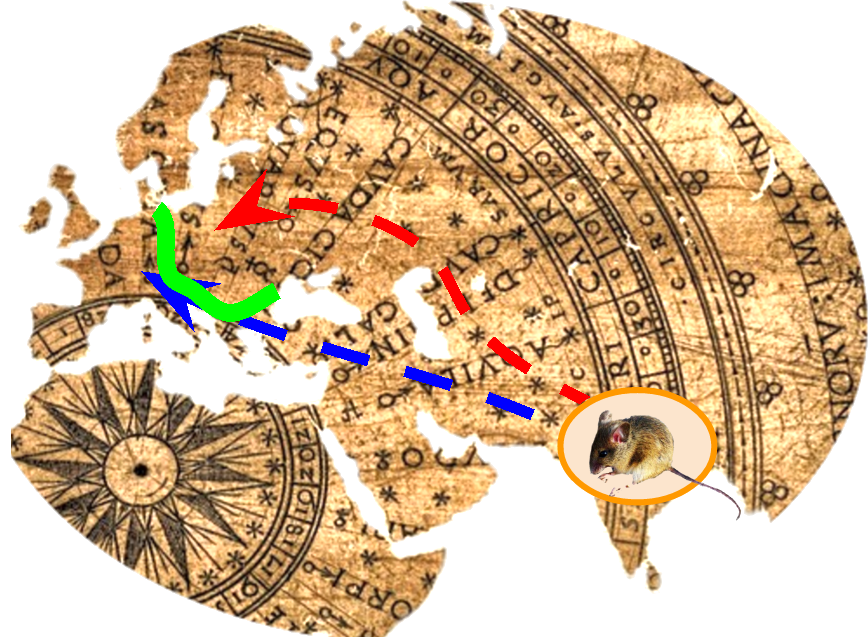
\includegraphics[scale=0.6]{R7.png}
\end{tikzfigure}
 
       
        \end{itemize}
}

% AIMS
% ----

\block{Aims of the study}
{
	\begin{enumerate}
	\item Investigate the \textbf{hybrid vigor/resistance} of house mouse to their parasite \textit{Eimeria}~spp. using prevalence and intensity data for parasite strains throughout the House Mouse Hybrid Zone
	\item Test \textbf{local adaptation} between the host and its parasite
	\end{enumerate}
}


% Material \& Methods: Field study
% -------
\block{Material \& Methods: Field study}
{
\begin{tikzfigure}[Annual sampling every September. Oocyst counted in mice feces. Mice assigned to a hybrid index based on \textit{M.m.domesticus}/\textit{M.m.musculus} alleles ratio (Machol\'{a}n \textit{et al.} (2011) )]
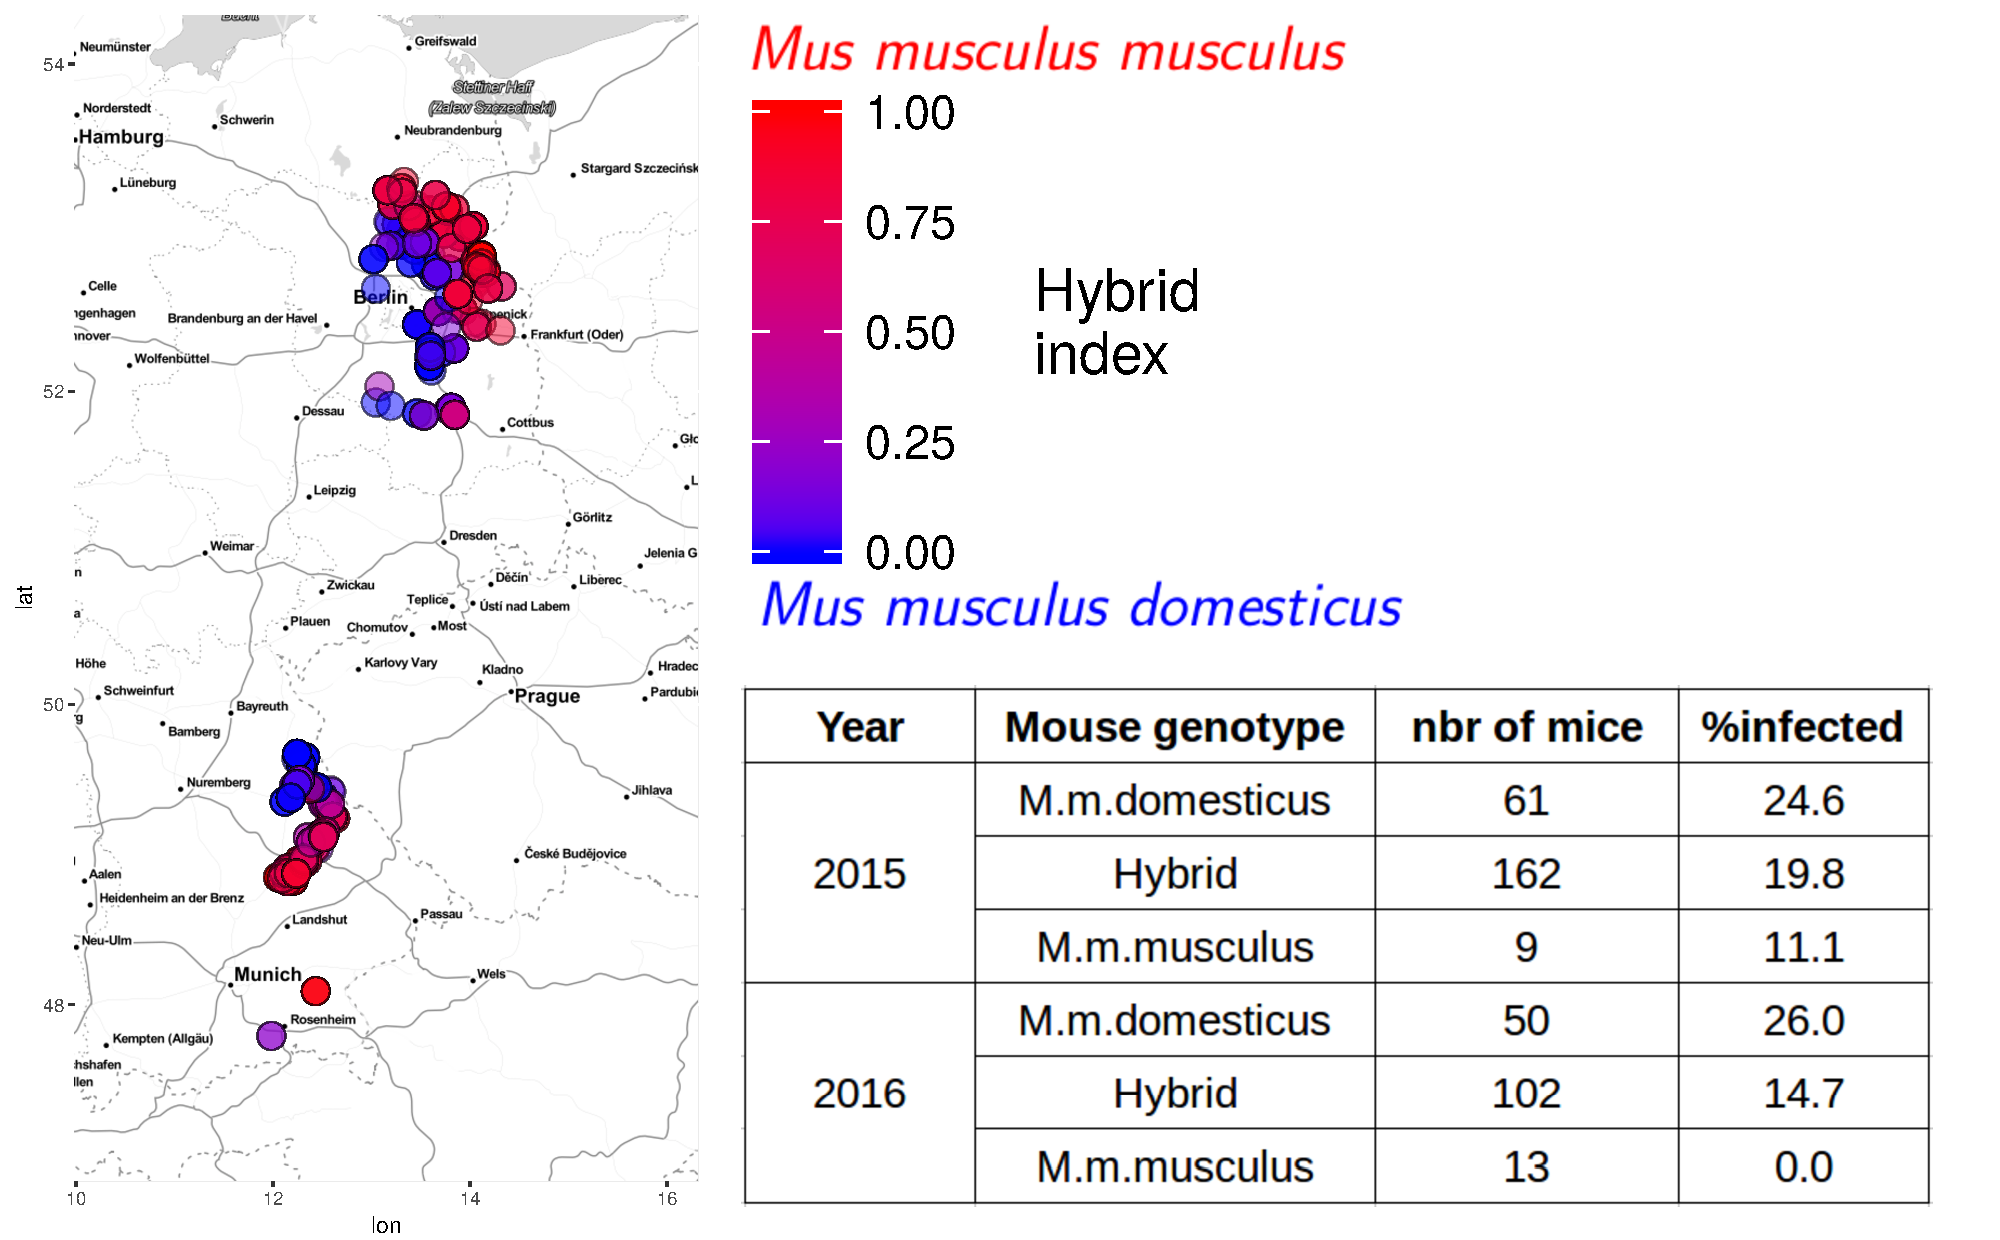
\includegraphics[scale=1]{map.pdf}
\end{tikzfigure}

    }

% Material \& Methods: Cross infection
% -------

\block{Material \& Methods: Cross infection}
      {
      \begin{itemize}
      
      \item Parasite strains:
      
      \begin{enumerate}
      \item \textbf{\textit{Eimeria} A} laboratory strain \textit{Eimeria falciformis} (Heitlinger \textit{et al.} 2014)
      \item \textbf{\textit{Eimeria} B} strain isolated in the wild 
      \end{enumerate}
      
      \item Host strains:
      
      \begin{enumerate}
      \item \textbf{WSB} Wild-derived inbred strain. Derived from wild \textit{Mus musculus domesticus}\\ Region of capture: Eastern Shore, Maryland
      \item \textbf{PWD} Wild-derived inbred strain. Derived from wild \textit{Mus musculus musculus}\\ Region of capture: near Prague, Czech Republic
      \item \textbf{WP} Hybrids between the two previous strains
      \end{enumerate}
      
      \end{itemize}
}


      % ACKNOWLEDGEMENTS
% ----------------
      \note[targetoffsetx=-13cm, targetoffsety=-13cm, width=28cm, innersep=0cm]
{
    \begin{wrapfigure}{r}{3cm}	
   \vspace{-90pt}
   
	
\includegraphics[scale=0.30]{Logos.png}
	
	\end{wrapfigure}
	\textbf{Funding:} This research has received funding 
	from the DFG, and is part of a IZW/HU project\\
        A. Balard is part of the Dahlem Research School
}


% ------------------------
% COLUMN 2 ---------------

\column{0.5}

\block{Exploring hybrid vigor/resistance in the wild}
{

\vfill
  \item Adaptation of the method of Stuart J.E. Baird (Baird \textit{et al.} 2012): \\ Maximum likelihood analysis explicitly linking parasite abundance to a gradient along the hybrid index as a proxy of host heterozygosity  \vspace{+1ex}
  
\begin{tikzfigure}[Generalized linear model with negative binomial distribution: \textbf{glm.hybrid} applied to simulated data, two groups both presenting a hybrid vigor]
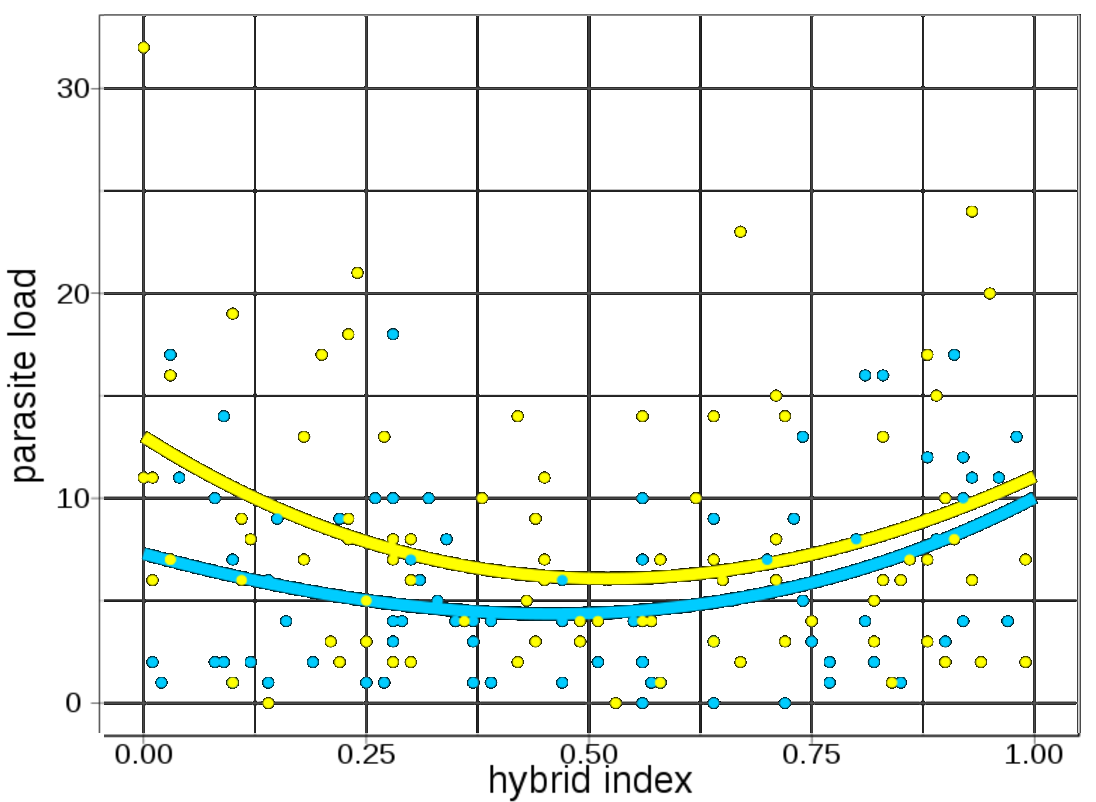
\includegraphics[scale=0.5]{model.png}
\end{tikzfigure}

      \item R package under development: \url{https://github.com/alicebalard/Parasite_Load}
\textbf{Goal: using our glm.hybrid model to assess the existence of hybrid vigor/resistance, taking into account the parasite strains}
      \textcolor{blue}{\[Parasite\ load \sim mouse\ heterozygosity\ level * parasite\ strain  \]}\vspace{-2ex}% reduce space

}

% PART II 
% -------

\block{Results of the infection experiment}
{ 
  \begin{itemize}
    \item \textit{Eimeria} B has \textbf{lower parasite shedding} and \textbf{lower relative weight retained} in mice strains WSB compared to PWD 
    \item \textit{Eimeria} B has \textbf{lower parasite shedding} and \textbf{lower relative weight retained} in mice hybrids than in the pure strains
  \end{itemize}

\begin{tikzfigure}[First indications of \textbf{local adaptation} and \textbf{hybrid vigor}]
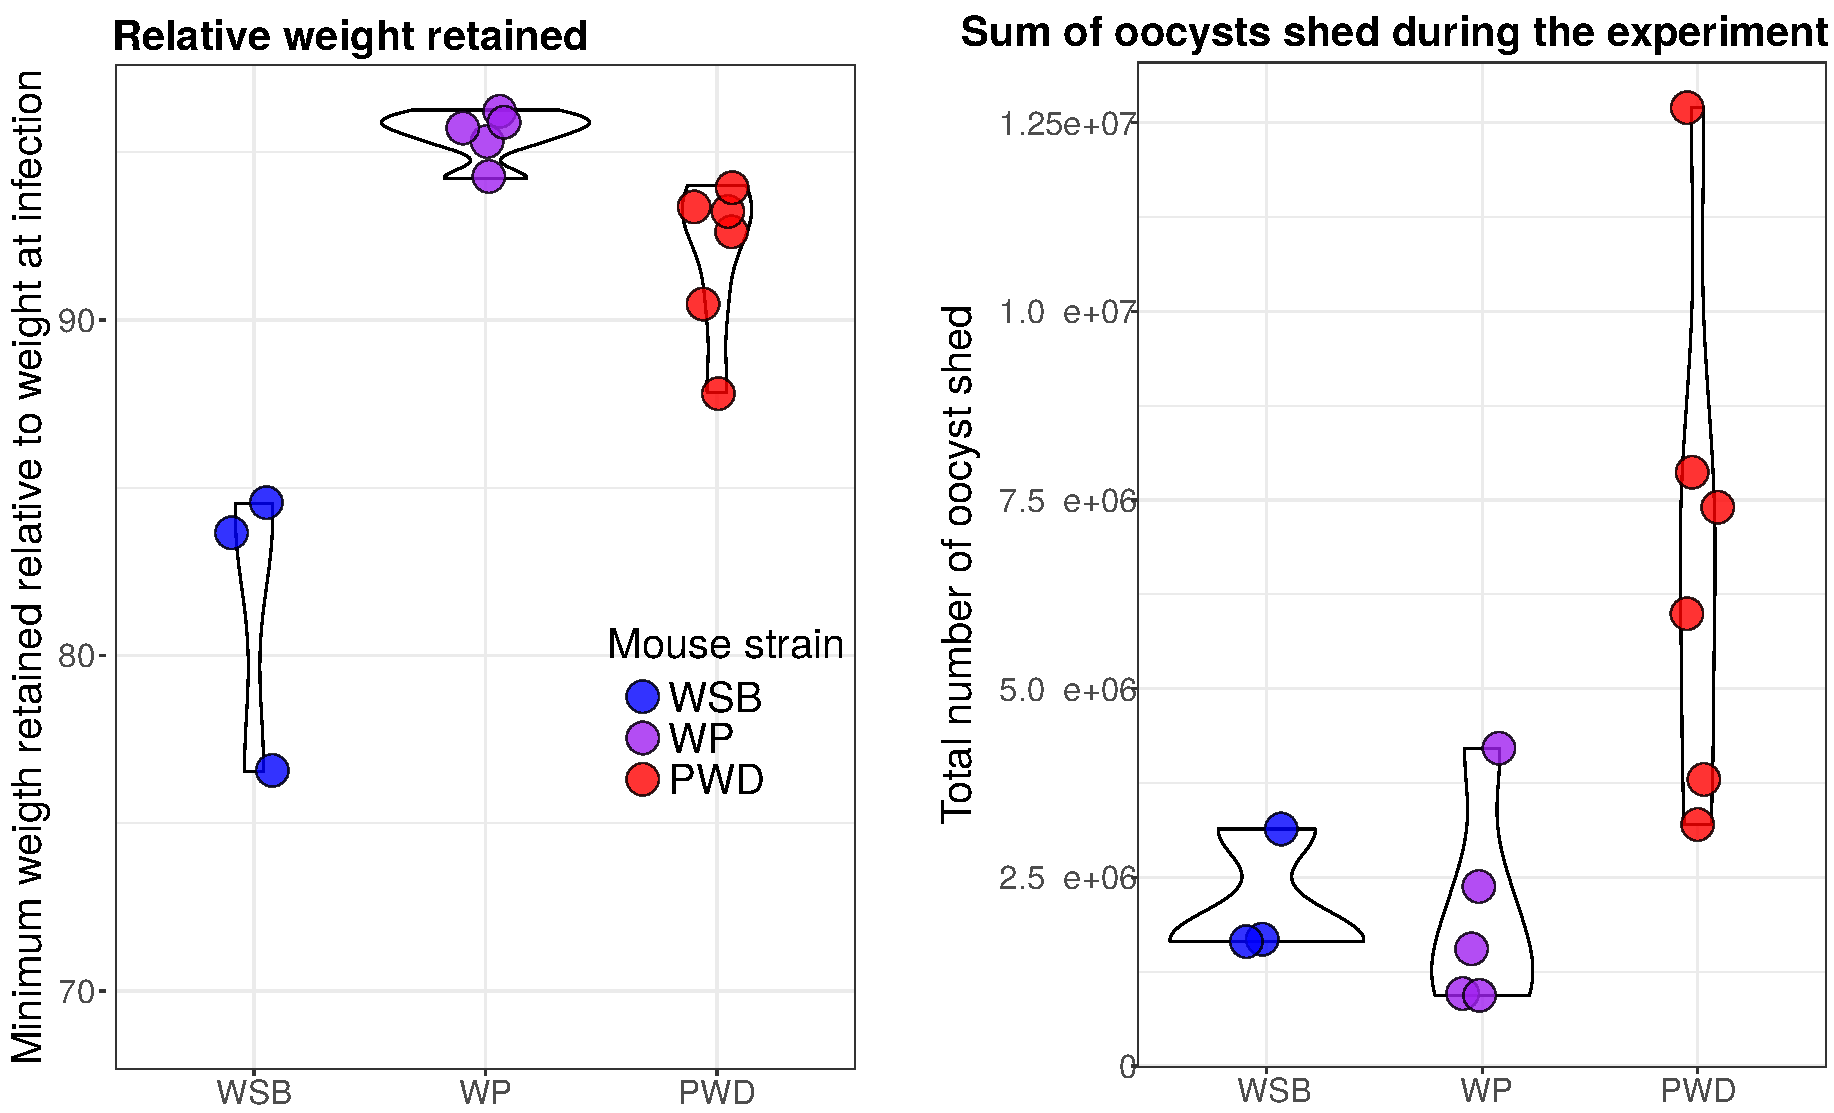
\includegraphics[scale=1]{May2017_E64.pdf}
\end{tikzfigure}

}

\block{Perspective}
{
  Next cross infection experiment: 
%  \begin{center}
    \begin{itemize}
        \item Test our hypotheses of hybrid vigor (within subspecies heterosis vs between subspecies)
        \item Assess local adaptation in other parasite strains
  \end{itemize}

 % \end{center}
 Field data:
    \begin{itemize}
        \item Obtain enough data (Sept. 2017) to test our hypotheses of hybrid vigor and local adaptation in the wild
  \end{itemize}

 
}

% REFERENCES
% ----------

\block{References}
      {
        \begin{small}
          
          \hangindent=2cm Baird \textit{et al.} (2012) Where Are the Wormy Mice? A Reexamination of Hybrid Parasitism in the European House Mouse Hybrid Zone \textit{Evolution} 66 (9): 2757--72
           
          \hangindent=2cm Heitlinger \textit{et al.} (2014) The genome of Eimeria falciformis-reduction and specialization in a single host apicomplexan parasite \\ \textit{BMC genomics} 15 (1), 696
          
          \hangindent=2cm Machol\'{a}n \textit{et al.} (2011) Assessing Multilocus Introgression Patterns: A Case Study on the Mouse X Chromosome in Central Europe \textit{Evolution} 65: 1428--1446

          \hangindent=2cm Machol\'{a}n \textit{et al.} (2012) Evolution of the House Mouse
          \textit{Cambridge University Press}
          
        
          
        \end{small}
      }

\end{columns}

% ----------------
\end{document}
\endinput
%%
%% End of file 
